\documentclass{article}
% Recommended, but optional, packages for figures and better typesetting:
\usepackage{amsmath}
\usepackage{microtype}
\usepackage{graphicx}
\usepackage{subfigure}
\usepackage{algorithm}
\usepackage{algorithmic}
\usepackage{booktabs}
\usepackage{hyperref}
\usepackage[accepted]{icml2025}
\usepackage{amsmath}
\usepackage{amssymb}
\usepackage{mathtools}
\usepackage{amsthm}
\usepackage{xurl}
\usepackage[capitalize,noabbrev]{cleveref}

%%%%%%%%%%%%%%%%%%%%%%%%%%%%%%%%
% THEOREMS
%%%%%%%%%%%%%%%%%%%%%%%%%%%%%%%%
\theoremstyle{plain}
\newtheorem{theorem}{Theorem}[section]
\newtheorem{proposition}[theorem]{Proposition}
\newtheorem{lemma}[theorem]{Lemma}
\newtheorem{corollary}[theorem]{Corollary}
\theoremstyle{definition}
\newtheorem{definition}[theorem]{Definition}
\newtheorem{assumption}[theorem]{Assumption}
\theoremstyle{remark}
\newtheorem{remark}[theorem]{Remark}

\usepackage[textsize=tiny]{todonotes}

\begin{document}
\icmltitlerunning{\icmltitlerunning{Knowledge Distillation for Efficient On-Device Image Classification}}
\twocolumn[
\icmltitle{Knowledge Distillation for Efficient On-Device Image Classification}

\icmlsetsymbol{equal}{*}

\begin{icmlauthorlist}
\icmlauthor{Abdul Hafeez (25280098)}{lums}
\icmlauthor{Verda Batool (24280065)}{lums}
\icmlauthor{Saad Ali (25280011)}{lums}
\end{icmlauthorlist}

\icmlaffiliation{lums}{Department of Electrical Engineering, Lahore University of Management Sciences, Lahore, Pakistan}

\icmlcorrespondingauthor{Saad Ali}{25280011@lums.edu.pk}

\icmlkeywords{Knowledge Distillation, Model Compression, On-Device Deep Learning, CIFAR-100, ResNet, Temperature Scaling, Ablation Study}
\vskip 0.3in
]

\noindent\textbf{Code:} \url{https://github.com/saadali18/on-device-image-classification}\\


% ========================================================================
\begin{abstract}
Deploying accurate image classifiers on resource-constrained edge devices requires compact models that preserve most of a large model's accuracy. We study response-based knowledge distillation \citep{hinton2015distilling} as a principled compression strategy on CIFAR-100, using a pretrained ResNet-110 teacher ($73.48\%$ Test Top-1) to supervise a family of smaller students via a combined hard-label cross-entropy and temperature-scaled KL divergence objective. Against a hard-label ResNet-20 baseline of $67.63\%$ Test Top-1, our temperature sweep $\tau \in \{2, 4, 8, 16\}$ and loss-weighting sweep $\alpha \in \{0.1, 0.5, 0.9\}$ both exhibit clean inverted-U behaviour with peaks at $\tau^* = 8$ and $\alpha^* = 0.5$. An architectural-scaling sweep across depth (ResNet-$\{20, 32, 44, 56\}$) and width ($w \in \{0.5, 1, 2\}$) shows that distilled-student accuracy is monotonic in capacity in our regime: three of five capacity points exceed the teacher's accuracy, with the wider ResNet-20 ($w=2$, $1.10$M parameters --- still $1.6\times$ smaller than the teacher) reaching $\mathbf{75.43\%}$ Top-1, $\mathbf{+7.80}$ pp above the hard-label baseline and $\mathbf{+1.95}$ pp above the teacher itself. The contrary failure mode appears at the low-capacity end: ResNet-20 narrowed to $w=0.5$ ($72$k parameters) finishes $10.37$ pp \emph{below} baseline, demonstrating a minimum-capacity threshold below which dark knowledge cannot be absorbed. A distributional analysis visualises the teacher's softened logits and a calibration analysis reveals a non-obvious side-effect: distillation degrades calibration (ECE rises from $6.23\%$ to $\sim 10\%$) as the student inherits the teacher's overconfidence pattern.
\end{abstract}
% ========================================================================

\section{Introduction}
\label{sec:intro}
Deep Convolutional Neural Networks (CNNs) like ResNet-110 achieve state-of-the-art accuracy in an over-parameterized regime ($\approx$1.7M parameters) \citep{he2016deep}, but deployment to edge devices enforces hard constraints on memory and inference latency that such models violate. \citet{compression2006} introduced model compression as a principled solution; \citet{hinton2015distilling} formalized this as \emph{Knowledge Distillation} (KD) for neural networks.

In standard $K$-class classification, a network produces logits $z_k$ passed through softmax
\begin{equation}
  \hat{y}_k = \frac{e^{z_k}}{\sum_{j=1}^K e^{z_j}},
  \label{eq:softmax}
\end{equation}
optimized via categorical cross-entropy against one-hot labels $\vec{y}_i \in \{0,1\}^K$:
\begin{equation}
    L = -\frac{1}{N}\sum_{i=1}^N \sum_{k=1}^K y_{i,k} \log(\hat{y}_{i,k}).
    \label{eq:cce}
\end{equation}
Hard labels discard inter-class similarity. A large teacher network\footnote{We use superscripts $T$ and $S$ to denote teacher and student quantities respectively.} trained to near-convergence absorbs this structure into its output distribution $\hat{\vec{y}}^T$, placing small but nonzero probabilities on semantically related classes --- \emph{dark knowledge} \citep{hinton2015distilling}. KD incorporates $\hat{\vec{y}}^T$ directly into the student's training objective, exposing this richer supervision signal. This project studies that transfer: \emph{what} the teacher transfers, how hyperparameters control it, and where it fails.

\section{Literature Review}
\label{sec:litreview}
\subsection{Model Compression Landscape}
\label{sec:compression}

Model compression falls into three families \citep{gou2021knowledge}: (i) \emph{Pruning} removes weights or filters from a pretrained network \citep{cheng2024surveydeepneuralnetwork}; (ii) \emph{Quantization} reduces numerical precision (e.g.\ FP32 → INT8) to shrink memory and accelerate arithmetic \citep{nagel2021whitepaperneuralnetwork}; (iii) \emph{Distillation} trains a new compact student network supervised by a larger teacher. All three are mutually compatible and frequently pipelined. This paper is scoped to response-based distillation, which transfers knowledge through the teacher's output distribution.

\subsection{Response-Based Distillation}
\label{sec:hinton}
\paragraph{The hard-label gradient problem.}
The gradient of Eq.~\eqref{eq:cce} with respect to the student's pre-softmax logit $z_k^S$ is
\begin{equation}
  \frac{\partial L}{\partial z_k^S} = \hat{y}_k^S - y_k.
  \label{eq:cce_grad}
\end{equation}
For every non-target class $y_k = 0$, so the update becomes
$z_k^S \leftarrow z_k^S - \eta\hat{y}_k^S$,
strictly pushing non-target logits toward $-\infty$ regardless 
of class similarity.

\paragraph{Temperature scaling.}
\citet{hinton2015distilling} introduced the temperature-scaled softmax: for teacher logits $\vec{z}^T$,
\begin{equation}
\hat{y}_k^{T,\tau} = \frac{\exp(z_k^T / \tau)}{\sum_{j=1}^K \exp(z_j^T / \tau)},
\label{eq:softtarget}
\end{equation}
applied equally to the student to produce $\hat{y}_k^{S,\tau}$. Increasing $\tau > 1$ softens the distribution, amplifying the relative magnitude of non-target class gradients and exposing inter-class similarity to the student. At $\tau\!\to\!\infty$ the distribution approaches uniform; at $\tau\!\to\!0$ it collapses to a one-hot argmax.

\paragraph{Training objective.}
The student optimizes a weighted sum of a hard-label term,
\begin{equation}
  L_{\mathrm{hard}}
    = -\frac{1}{N}\sum_{i=1}^N\sum_{k=1}^K
        y_{i,k}\log\hat{y}_{i,k}^{S,1},
  \label{eq:lhard}
\end{equation}
and a soft-label KL divergence term,
\begin{equation}
  L_{\mathrm{soft}}
    = \frac{1}{N}\sum_{i=1}^N
        D_{\mathrm{KL}}\!\left(
          \hat{\vec{y}}_i^{T,\tau}
          \,\Big\|\,
          \hat{\vec{y}}_i^{S,\tau}
        \right).
  \label{eq:lsoft}
\end{equation}
Expanding and grouping by entropy terms gives
\begin{equation*}
  L_{\mathrm{soft}} = H(\hat{\vec{y}}^{T,\tau},\,\hat{\vec{y}}^{S,\tau}) - H(\hat{\vec{y}}^{T,\tau}).
\end{equation*}
Since the teacher is frozen, $H(\hat{\vec{y}}^{T,\tau})$ is constant w.r.t.\ the student, so minimizing $L_{\mathrm{soft}}$ is equivalent to minimizing the cross-entropy $H(\hat{\vec{y}}^{T,\tau}, \hat{\vec{y}}^{S,\tau})$.

\paragraph{The $\tau^2$ scaling factor.}
We defer the full gradient derivation to Appendix~\ref{app:tau2}; the result is $\partial L_{\mathrm{soft}}/\partial z_k^S = (z_k^S - z_k^T)/(K\tau^2)$, which scales as $1/\tau^2$ relative to the hard-label gradient. Without correction, raising $\tau$ shrinks the soft gradient as $1/\tau^2$, reverting the student to hard-label training; multiplying $L_{\mathrm{soft}}$ by $\tau^2$ cancels this shrinkage. The combined objective is:
%
\begin{equation}
  \boxed{
  L_{\mathrm{KD}}
    = \alpha \cdot L_{\mathrm{hard}}
    + (1-\alpha)\cdot\tau^2 \cdot L_{\mathrm{soft}}
  }
  \label{eq:lkd}
\end{equation}
where $\alpha \in [0,1]$ balances hard vs.\ soft supervision and $\tau$ controls distribution softness.

\section{Methodology}
\label{sec:method}

\paragraph{Dataset.} All experiments use CIFAR-100: 60{,}000 colour images at $32{\times}32$ across $K=100$ classes (50k train / 10k test).

\paragraph{Teacher.} ResNet-110 \citep{he2016deep} is trained from scratch on CIFAR-100 with standard cross-entropy for 160 epochs (LR milestones $\{80, 120\}$), then its weights are frozen for all distillation experiments. The longer schedule ensures the teacher converges to a high accuracy ceiling before being used as a soft-target source.

\paragraph{Student.} ResNet-20 \citep{he2016deep} ($\approx$0.27M parameters, $6.3\times$ smaller than the teacher) serves as the default student. It is architecturally homogeneous with ResNet-110, isolating depth as the primary capacity variable.

\subsection{Baseline and Student Variants}
\label{sec:baseline}
We train ResNet-20 from scratch with standard CCE (no teacher) to establish the lower bound for distillation to beat. For the capacity study we define two families: a \textit{depth} series ResNet-$d$, $d \in \{20, 32, 44, 56\}$ (width 16), and a \textit{width} series ResNet-20 with multiplier $w \in \{0.5, 1, 2\}$ (base channels $\{8, 16, 32\}$). The ResNet-20 ($w=1$) serves as the shared pivot.

\subsection{Training Configuration}
\label{sec:training_config}
\begin{table}[ht]
  \centering
  \caption{\textbf{Training configuration.} Teacher uses 160 epochs with milestones $\{80,120\}$; all else identical.\\}
  \label{tab:hyperparams}
  \begin{tabular}{lc}
    \toprule
    \textbf{Hyperparameter} & \textbf{Value} \\
    \midrule
    Optimiser            & SGD + Momentum (0.9) \\
    Initial LR           & 0.1 (MultiStep) \\
    LR milestones / $\gamma$ & epochs 60, 80 / 0.1 \\
    Weight decay         & $5\times10^{-4}$ \\
    Batch size / Epochs  & 128 / 100 \\
    Loss                 & Cross-entropy \\
    \bottomrule
  \end{tabular}
\end{table}

% ========================================================================
\section{Results}
\label{sec:results}

\subsection{Baseline and Teacher}
\label{sec:results_baseline_teacher}

Training ResNet-20 from scratch on CIFAR-100 establishes the lower bound; the ResNet-110 teacher uses the longer schedule in Section~\ref{sec:method}. Best-checkpoint metrics are in Table~\ref{tab:baseline}. The $73.48 - 67.63 = 5.85$ pp teacher--baseline gap defines the headroom available to distillation.

\begin{table}[ht]
  \centering
  \caption{
    \textbf{Baseline and teacher best-checkpoint metrics.}}
  \label{tab:baseline}
  \begin{tabular}{lcc}
    \toprule
    \textbf{Metric} & \textbf{Baseline} & \textbf{Teacher} \\
                    & \textbf{(ResNet-20)} & \textbf{(ResNet-110)} \\
    \midrule
    Parameters          & 278{,}324    & 1{,}736{,}564 \\
    Best Epoch          & 89           & 129 \\
    Test Top-1          & 67.63\%      & 73.48\% \\
    Test Top-5          & 91.31\%      & 92.74\% \\
    \bottomrule
  \end{tabular}
\end{table}

\subsection{Hyperparameter Ablation}
\label{sec:results_hparam}

\paragraph{Temperature.} Fixing $\alpha = 0.5$, we sweep $\tau \in \{2, 4, 8, 16\}$ (Table~\ref{tab:tau_sweep}). The sweep produces a clean inverted-U peaking at $\tau^* = 8$, recovering $40\%$ of the teacher--baseline gap at zero parameter cost.

\begin{table}[ht]
  \centering
  \caption{\textbf{Temperature ablation} ($\alpha=0.5$, ResNet-20, 100 epochs).}
  \label{tab:tau_sweep}
  \begin{tabular}{ccc}
    \toprule
    $\tau$ & Test Top-1 & $\Delta$ vs.\ baseline \\
    \midrule
    2  & 69.49\% & $+1.86$ \\
    4  & 69.64\% & $+2.01$ \\
    \textbf{8}  & \textbf{69.98\%} & $\mathbf{+2.35}$ \\
    16 & 69.73\% & $+2.10$ \\
    \bottomrule
  \end{tabular}
\end{table}

\paragraph{Loss weighting.} Using $\tau^* = 8$, we sweep $\alpha \in \{0.1, 0.5, 0.9\}$ (Table~\ref{tab:alpha_sweep}). All three values improve over the baseline; the balanced $\alpha^* = 0.5$ is optimal, with $\alpha=0.9$ recovering only $62\%$ of the gain --- confirming the soft-label term does real work.

\begin{table}[ht]
  \centering
  \caption{\textbf{Loss-weighting ablation} ($\tau = 8$, ResNet-20, 100 epochs).}
  \label{tab:alpha_sweep}
  \begin{tabular}{ccc}
    \toprule
    $\alpha$ & Test Top-1 & $\Delta$ vs.\ baseline \\
    \midrule
    0.1 & 69.74\% & $+2.11$ \\
    \textbf{0.5} & \textbf{69.98\%} & $\mathbf{+2.35}$ \\
    0.9 & 69.07\% & $+1.44$ \\
    \bottomrule
  \end{tabular}
\end{table}

\subsection{Architectural Scaling}
\label{sec:results_arch}

Using $(\tau^*, \alpha^*) = (8, 0.5)$, we measure distillation benefit along depth and width axes.

\paragraph{Depth.} Table~\ref{tab:depth_sweep} sweeps ResNet-$d$, $d \in \{20, 32, 44, 56\}$ at width $w=1$.

\begin{table}[ht]
  \centering
  \caption{\textbf{Depth ablation} ($\tau=8$, $\alpha=0.5$, 100 epochs). $\Delta_{\text{T}}$: gap vs.\ teacher (73.48\%).}
  \label{tab:depth_sweep}
  \begin{tabular}{lcccc}
    \toprule
    Student & Params & Top-1 & $\Delta$ base & $\Delta_{\text{T}}$ \\
    \midrule
    ResNet-20 & 278{,}324 & 69.98\% & $+2.35$ & $-3.50$ \\
    ResNet-32 & 472{,}756 & 72.39\% & $+4.76$ & $-1.09$ \\
    ResNet-44 & 667{,}188 & 73.52\% & $+5.89$ & $+0.04$ \\
    \textbf{ResNet-56} & 861{,}620 & \textbf{74.72\%} & $\mathbf{+7.09}$ & $\mathbf{+1.24}$ \\
    \bottomrule
  \end{tabular}
\end{table}

\paragraph{Width.} Table~\ref{tab:width_sweep} sweeps $w \in \{0.5, 1, 2\}$ at depth 20.

\begin{table}[ht]
  \centering
  \caption{\textbf{Width ablation} (ResNet-20, $\tau=8$, $\alpha=0.5$, 100 epochs). $\Delta_{\text{T}}$: gap vs.\ teacher.}
  \label{tab:width_sweep}
  \begin{tabular}{ccccc}
    \toprule
    $w$ & Params & Top-1 & $\Delta$ base & $\Delta_{\text{T}}$ \\
    \midrule
    0.5 &    71{,}756 & 57.26\% & $-10.37$ & $-16.22$ \\
    1.0 &   278{,}324 & 69.98\% & $+2.35$  & $-3.50$ \\
    \textbf{2.0} & 1{,}096{,}196 & \textbf{75.43\%} & $\mathbf{+7.80}$ & $\mathbf{+1.95}$ \\
    \bottomrule
  \end{tabular}
\end{table}

\begin{figure}[ht]
  \centering
  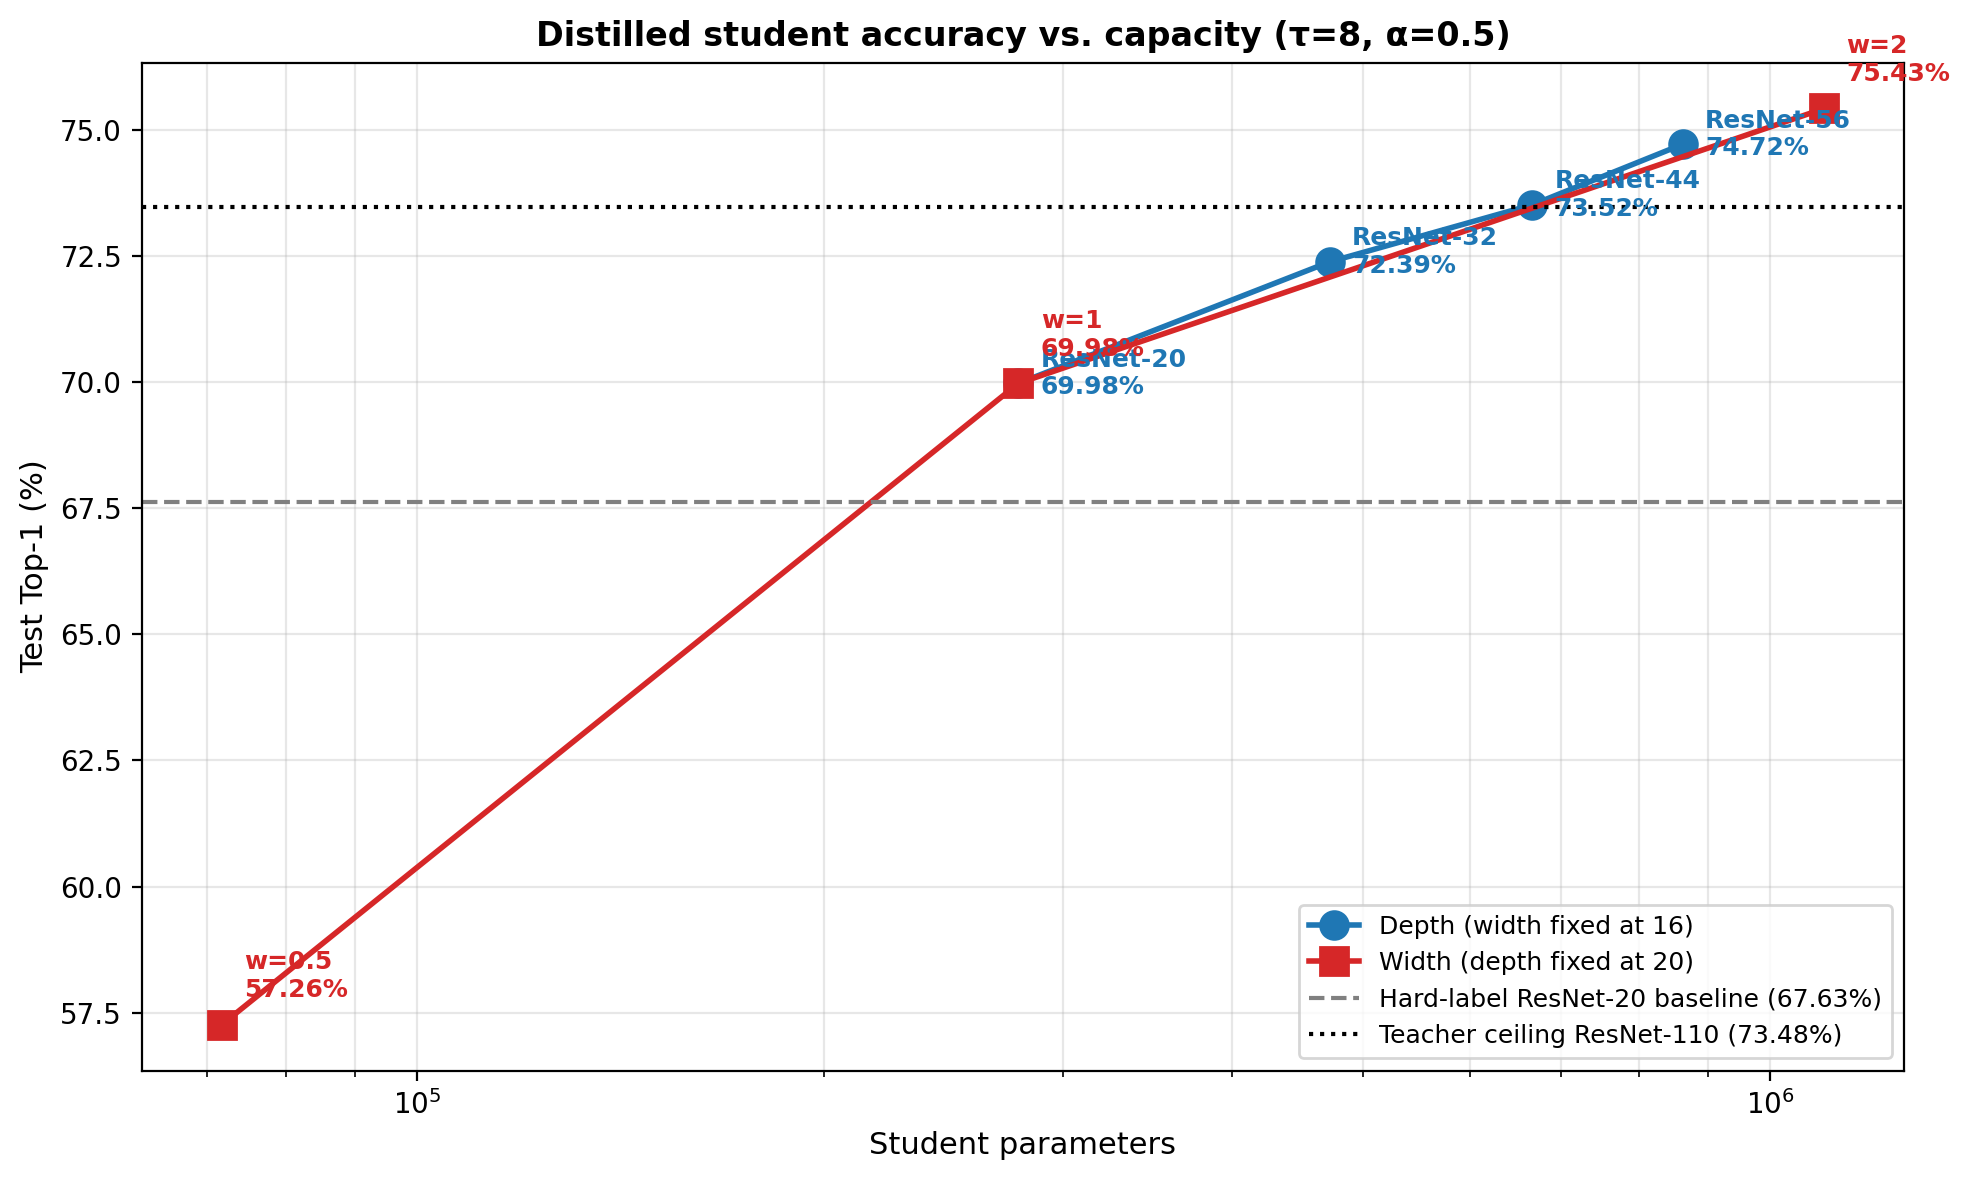
\includegraphics[width=\columnwidth]{../plots/analysis/capacity.png}
  \caption{
    \textbf{Distilled accuracy vs.\ capacity} ($\tau=8$, $\alpha=0.5$). Blue circles: depth series; red squares: width series. Gray/black lines: baseline and teacher.
  }
  \label{fig:capacity}
\end{figure}

% ========================================================================
\section{Dark Knowledge Analysis}
\label{sec:dark_knowledge}
Figure~\ref{fig:dark_knowledge} shows, for six held-out test images, the teacher's softmax distribution at $T=1$ and $T=4$.\footnote{Training used $\tau^*=8$; $T=4$ gives a more legible bar plot with identical top-$k$ ordering.} At $T=1$ the teacher's distribution is near one-hot; at $T=4$ it spreads tens of percentage points of mass onto semantically related classes. This off-argmax structure --- \emph{dark knowledge} \citep{hinton2015distilling} --- tells the student not just \emph{which} class is correct but \emph{how} the teacher's representation organises the class manifold, explaining the accuracy gains from distillation.

\begin{figure*}[ht]
  \centering
  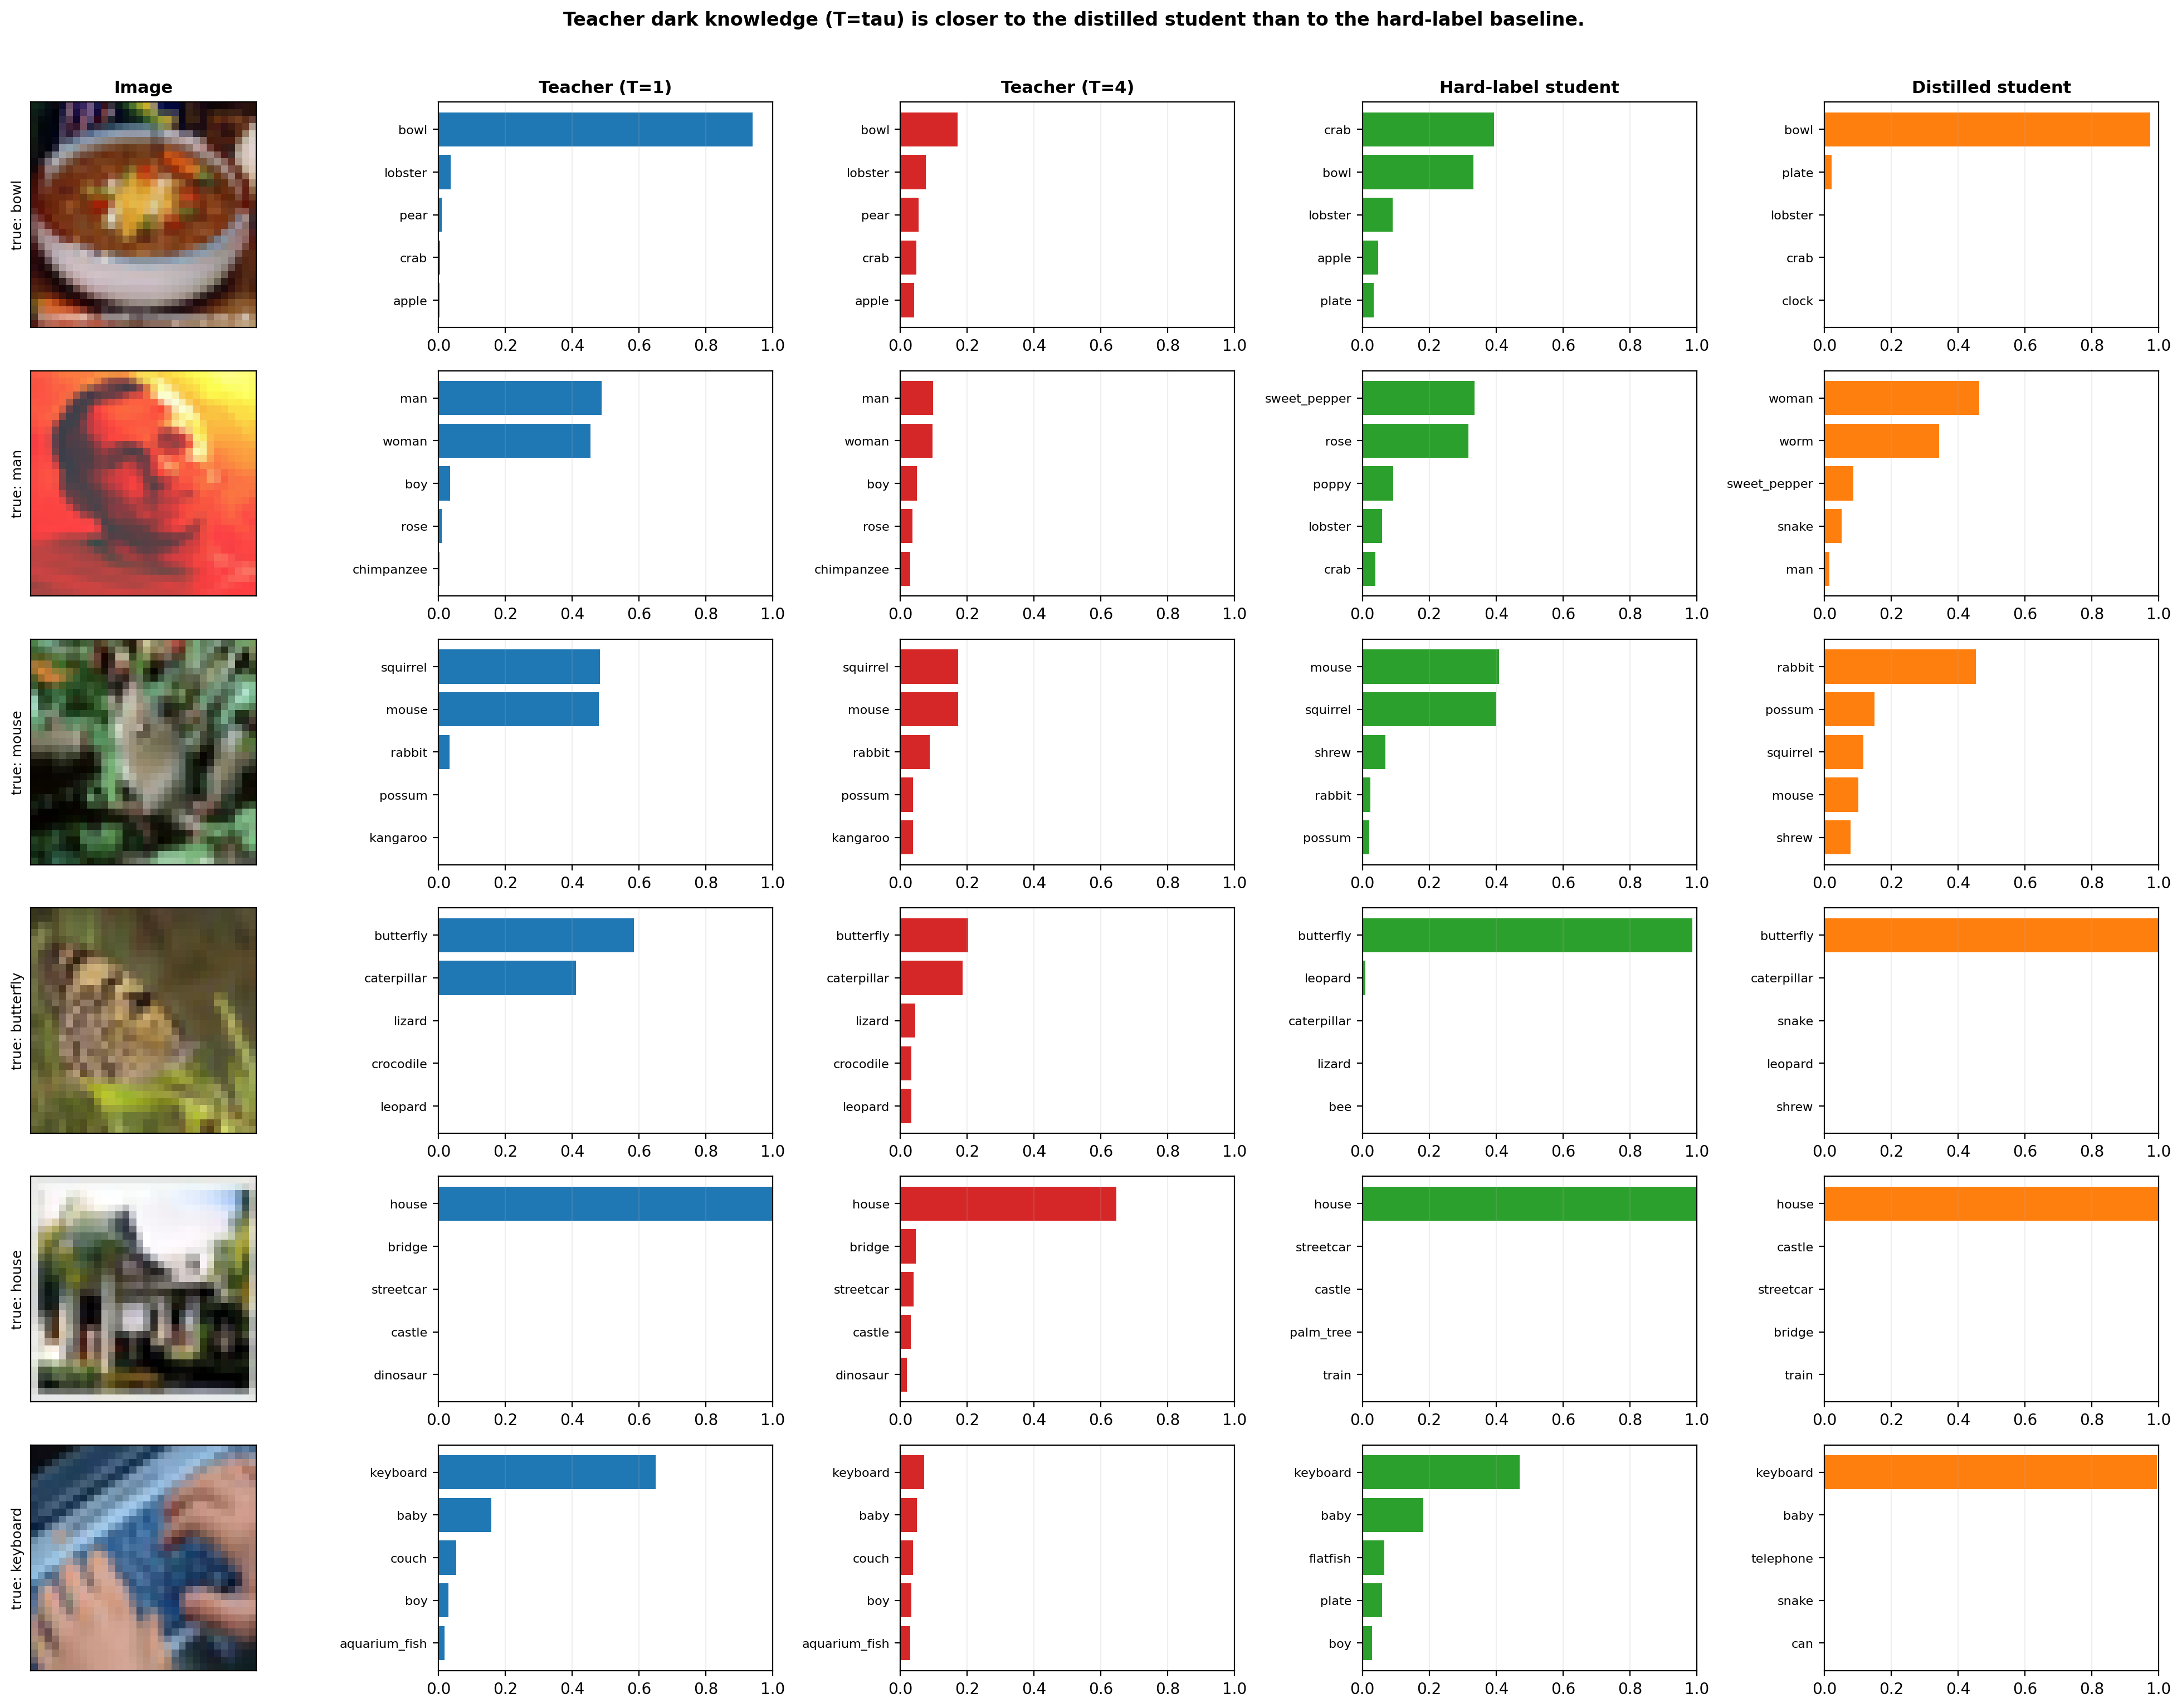
\includegraphics[width=\textwidth]{../plots/analysis/dark_knowledge.png}
  \caption{
    \textbf{Teacher dark knowledge.} Each row: input image; teacher softmax at $T{=}1$; teacher softmax at $T{=}4$; hard-label baseline student; distilled student. The softened teacher (red) reveals the inter-class similarity structure transferred by the distillation loss.
  }
  \label{fig:dark_knowledge}
\end{figure*}

% ========================================================================
\section{Calibration Analysis}
\label{sec:calibration}
Table~\ref{tab:calibration} reports Expected Calibration Error (ECE, 15 bins) and mean max-confidence $\bar{p}_{\max}$ on the CIFAR-100 test set; reliability diagrams are in Figure~\ref{fig:calibration}.

\begin{table}[ht]
  \centering
  \caption{\textbf{Calibration on CIFAR-100 test set} (ECE, 15 bins).}
  \label{tab:calibration}
  \begin{tabular}{lccc}
    \toprule
    Model & Top-1 & ECE & $\bar{p}_{\max}$ \\
    \midrule
    Teacher (ResNet-110)     & 73.48\% & 12.54\% & 0.860 \\
    Hard-label student       & 67.63\% & \textbf{6.23\%}  & 0.738 \\
    Distilled ($\tau{=}8$, $\alpha{=}0.5$) & 69.98\% & 10.32\% & 0.803 \\
    Distilled ($w{=}2$, best)& 75.43\% & 9.97\% & 0.854 \\
    \bottomrule
  \end{tabular}
\end{table}

\begin{figure}[ht]
  \centering
  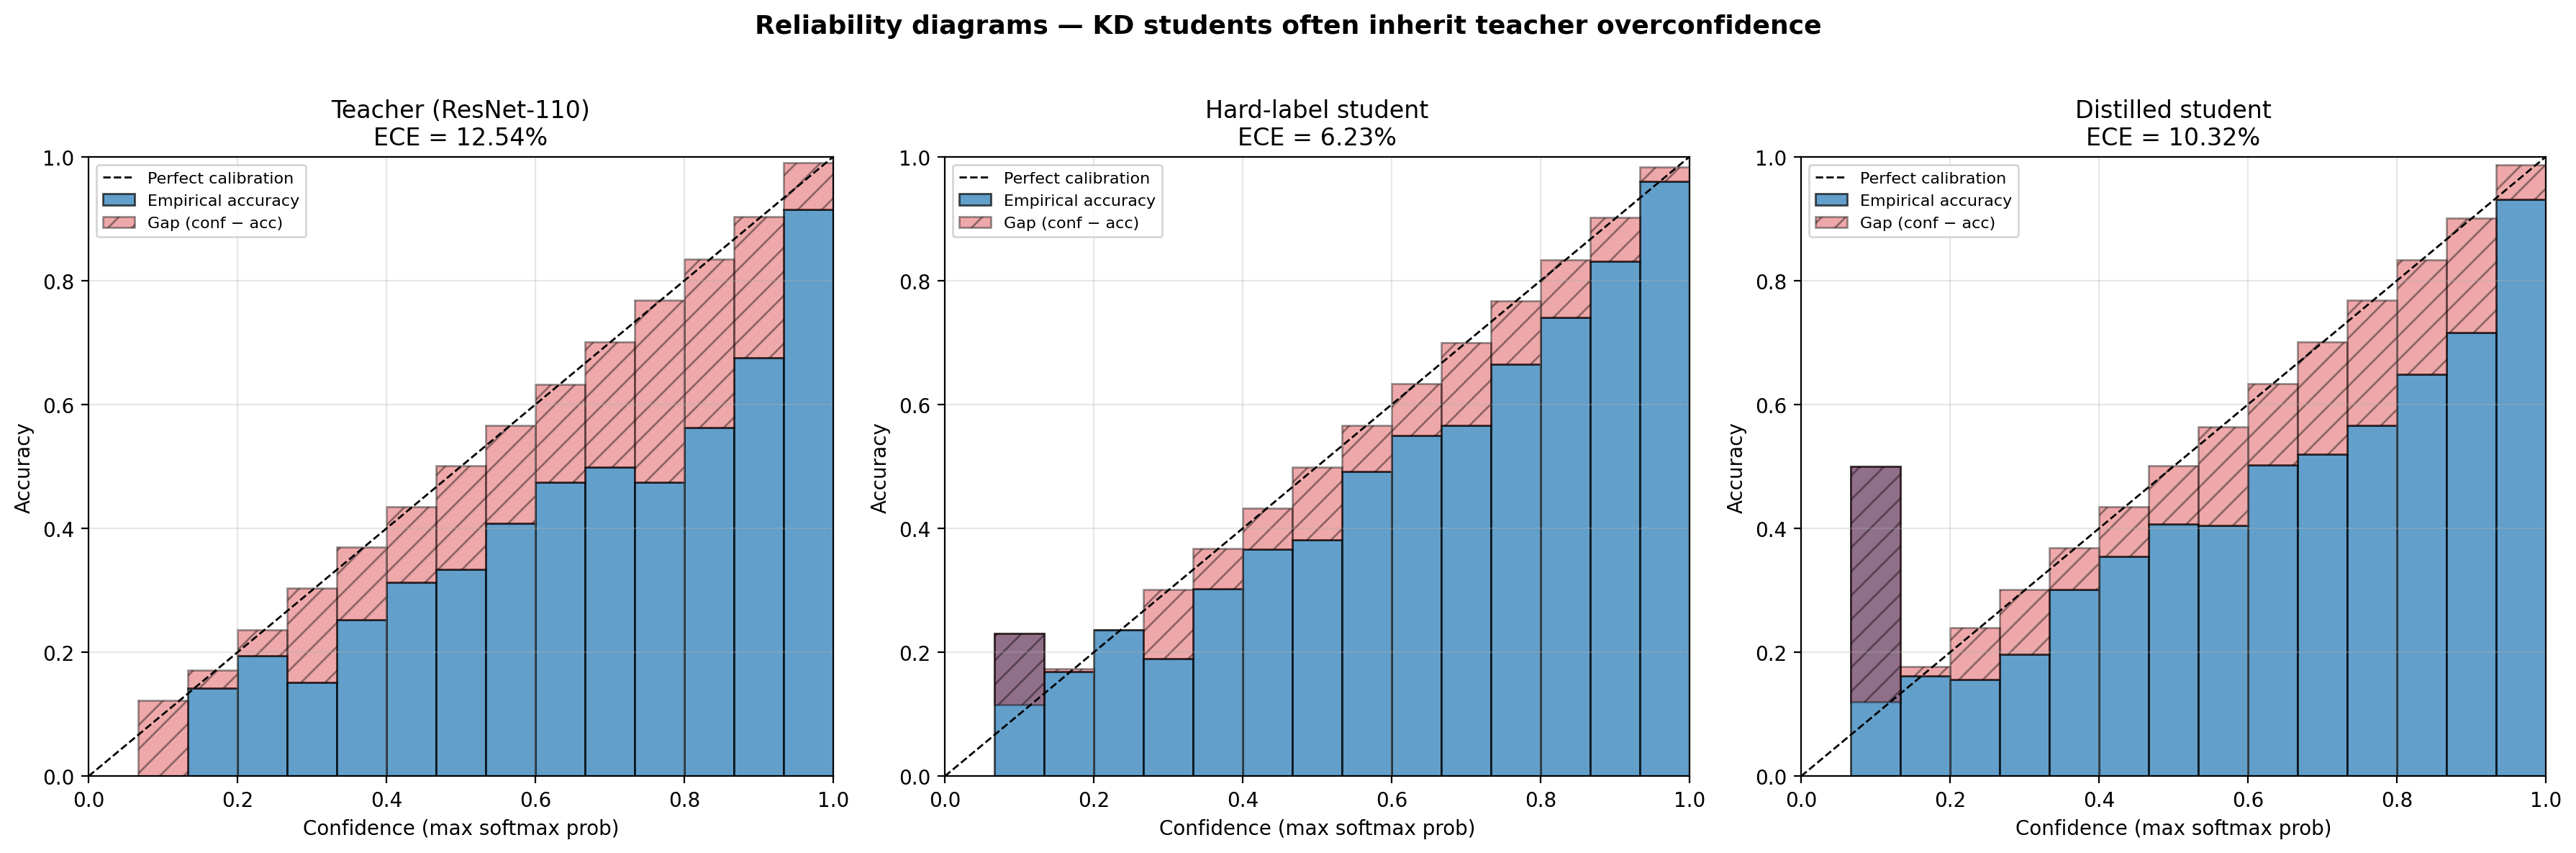
\includegraphics[width=\columnwidth]{../plots/analysis/calibration.png}
  \caption{
    \textbf{Reliability diagrams (15 bins).} The hard-label baseline is the best-calibrated model; distilled students inherit the teacher's overconfidence.
  }
  \label{fig:calibration}
\end{figure}

Counter-intuitively, the hard-label student (ECE $6.23\%$) is better calibrated than both distilled students despite lower Top-1 accuracy. The KL term transfers the teacher's full output distribution---including its overconfidence profile ($\bar{p}_{\max}=0.860$)---so the distilled student's confidence shifts toward the teacher's, raising ECE to ${\sim}10\%$. Accuracy and calibration are not jointly improved by KD; post-hoc calibration is required for probability-sensitive downstream tasks.

% ========================================================================
\section{Discussion}
\label{sec:discussion}

\paragraph{Temperature traces a clean inverted-U.}
The $\tau$ sweep confirms KD theory: too-sharp distributions approach hard labels while too-flat distributions approach uniform, both eliminating discriminative signal. $\tau^* = 8$ exceeds Hinton's canonical $\tau \approx 4$ because our ResNet-110 teacher retains $>40\%$ of mass on its argmax at $\tau=4$, requiring further softening to expose useful inter-class structure; with 100 classes, non-target logit gradients are also inherently small and benefit from the additional amplification.

\paragraph{$\alpha$ is less sensitive but still optimal at the balanced setting.}
All three $\alpha$ values improve over the baseline ($+1.44$--$+2.35$ pp), but the inverted-U peaks at $\alpha^* = 0.5$. The $\alpha=0.9$ deterioration (only $62\%$ of peak gain) rules out a pure-regularisation explanation, confirming the soft-label term is supplying genuinely new information. Conversely, $\alpha=0.1$ remains competitive, showing ground-truth anchoring retains value even when the teacher dominates.

\paragraph{Capacity scaling: ``student exceeds teacher''.}
Monotone scaling holds throughout our regime: three of five students cross the teacher's $73.48\%$ ceiling because our teacher sits below the ResNet-CIFAR family ceiling (${\sim}76\%$), so its soft-label signal continues to carry useful regularization well into the high-capacity regime. The headline result is $\mathbf{75.43\%}$ Top-1 ($+7.80$ pp) at $1.10$M parameters --- still $1.6\times$ smaller than the teacher. The $w=0.5$ ($72$k param) cell demonstrates the lower-end failure mode ($-10.37$ pp below baseline): the student lacks capacity to absorb either the dark-knowledge or discriminative signal, and the mixed distillation loss becomes noisier than CE alone.

\paragraph{Accuracy and calibration are not jointly improved.}
Distillation degrades calibration (ECE rises from $6.23\%$ to $10.32\%$) even as it improves Top-1 by up to $+7.80$ pp. The KL term transfers the teacher's full output distribution---including its overconfidence profile---not merely the argmax. Applications requiring calibrated probabilities must pair KD with a post-hoc calibration step (e.g.\ temperature scaling on a validation split). Single-seed training and a below-ceiling teacher ($73.48\%$ vs.\ literature ${\sim}76\%$) are the primary limitations of this study.

% ========================================================================
\section{Conclusion}
\label{sec:conclusion}

We studied response-based knowledge distillation \citep{hinton2015distilling} on CIFAR-100, using a ResNet-110 teacher ($73.48\%$ Top-1) to supervise a $6.3\times$ smaller ResNet-20 student. Our principal findings:

\begin{enumerate}
\item \textbf{Distillation closes $40\%$ of the teacher--baseline gap at zero parameter cost.} The best distilled ResNet-20 ($\tau^*=8$, $\alpha^*=0.5$) reaches $69.98\%$, recovering $2.35$ of the $5.85$ pp gap.

\item \textbf{Temperature traces an inverted-U peaking at $\tau^*=8$.} This validates the theoretical prediction that too-sharp or too-flat distributions both lose discriminative signal; $\tau^*=8 > 4$ (Hinton) because our teacher has sharper logits and CIFAR-100 has 100 classes.

\item \textbf{Loss weighting is less sensitive but still favours $\alpha^*=0.5$.} All $\alpha$ values improve over baseline; $\alpha=0.9$ recovers only $62\%$ of peak gain, ruling out a pure-regularisation effect.

\item \textbf{Distilled students can exceed the teacher when capacity is sufficient.} Three of five Step-3 students surpass the teacher's ceiling, with the best ($w=2$) reaching $\mathbf{75.43\%}$ at $1.10$M params; the $w=0.5$ cell ($72$k params) falls $10.37$ pp below baseline.

\item \textbf{Distillation degrades calibration even as it improves accuracy.} ECE rises from $6.23\%$ (baseline) to $10.32\%$ as the KL term transfers the teacher's overconfidence profile; post-hoc calibration is required for probability-sensitive applications.

\item \textbf{Dark knowledge is directly observable.} Temperature-softened teacher distributions reveal inter-class similarity structure, and distilled student outputs are visibly closer to these distributions than to the hard-label baseline.
\end{enumerate}

Future work includes cross-architecture distillation (CNN to MobileNetV2), feature-based methods \citep{romero2015fitnets}, and combining KD with pruning or quantization.

% ========================================================================
\section*{Statement on the Use of AI Tools}
Claude Code was used for software scaffolding, debugging, and structural report drafts. All experimental design, results interpretation, and mathematical derivations were produced by the team.

% ========================================================================
\appendix
\section{Gradient of $L_{\mathrm{soft}}$ with Respect to $z_k^S$}
\label{app:tau2}

\citet{hinton2015distilling} argue that the soft-label loss in combined distillation loss must be weighted by $\tau^2$. To prove this to be the case, we differentiate $L_{\mathrm{soft}}$, defined in Eq.~\eqref{eq:lsoft}, with respect to a student logit $z_k^S$. The gradient for a single sample (dropping index $i$ for convenience) is, by chain rule,
\begin{equation}
  \frac{\partial L_{\mathrm{soft}}}{\partial z_k^S}
  = \sum_{j=1}^{K}
      \frac{\partial L_{\mathrm{soft}}}{\partial \hat{y}_j^{S,\tau}}
      \cdot
      \frac{\partial \hat{y}_j^{S,\tau}}{\partial z_k^S}.
  \label{eq:chain}
\end{equation}
We evaluate each term individually. Since the teacher terms are
constant with respect to $\theta_S$, applying the logarithmic quotient rule and differentiating $-\sum_j \hat{y}_j^{T,\tau}\log\hat{y}_j^{S,\tau}$ with respect to $\hat{y}_j^{S,\tau}$ gives
\begin{equation}
  \frac{\partial L_{\mathrm{soft}}}{\partial \hat{y}_j^{S,\tau}}
  = -\frac{\hat{y}_j^{T,\tau}}{\hat{y}_j^{S,\tau}}.
  \label{eq:factor1}
\end{equation}
The student probability $\hat{y}_j^{S,\tau}$ depends on $z_k^S$
only through the scaled pre-activation $a_k^S = z_k^S/\tau$, so
a further application of the chain rule gives
\begin{equation}
  \frac{\partial \hat{y}_j^{S,\tau}}{\partial z_k^S}
  = \frac{\partial \hat{y}_j^{S,\tau}}{\partial a_k^S}
    \cdot
    \underbrace{\frac{\partial a_k^S}{\partial z_k^S}}_{=\,1/\tau},
  \label{eq:factor2_chain}
\end{equation}
where, by applying the quotient rule and considering the two distinct cases (diagonal and off-diagonal elements) for the jacobian,
\begin{equation}
  \frac{\partial \hat{y}_j^{S,\tau}}{\partial a_k^S}
  = \hat{y}_j^{S,\tau}\!\left(\delta_{jk} - \hat{y}_k^{S,\tau}\right).
  \label{eq:softmax_jac}
\end{equation}
Combining Eqs.~\eqref{eq:factor2_chain} and~\eqref{eq:softmax_jac} and substituting it along with Eq.~\eqref{eq:factor1} into Eq.~\eqref{eq:chain}
\begin{align}
  \frac{\partial L_{\mathrm{soft}}}{\partial z_k^S}
  &= \sum_{j=1}^{K}
      \left(-\frac{\hat{y}_j^{T,\tau}}{\hat{y}_j^{S,\tau}}\right)
      \cdot
      \frac{1}{\tau}\,\hat{y}_j^{S,\tau}
        \!\left(\delta_{jk} - \hat{y}_k^{S,\tau}\right)
  \nonumber\\
  &= \frac{1}{\tau}\sum_{j=1}^{K}
      \left(-\hat{y}_j^{T,\tau}\right)
        \!\left(\delta_{jk} - \hat{y}_k^{S,\tau}\right)
  \nonumber\\
  &= \frac{1}{\tau}\!\left[
      -\hat{y}_k^{T,\tau}
      + \hat{y}_k^{S,\tau}\underbrace{\sum_{j=1}^{K}
        \hat{y}_j^{T,\tau}}_{=\,1}
    \right]
  \nonumber\\
  &= \frac{1}{\tau}\!\left(\hat{y}_k^{S,\tau}
      - \hat{y}_k^{T,\tau}\right)
  \nonumber\\
  \intertext{Substituting Eq. \eqref{eq:softtarget}:}
  &= \frac{1}{\tau}\!\left(
        \frac{\exp(z_k^S/\tau)}{\sum_{j=1}^K \exp(z_j^S/\tau)}
        -
        \frac{\exp(z_k^T/\tau)}{\sum_{j=1}^K \exp(z_j^T/\tau)}
     \right)
  \nonumber\\
  \intertext{Applying first-order Taylor approximation $e^u \approx 1 + u$, valid when $\tau$ is large relative to the logit magnitudes \citep{hinton2015distilling}:}
  &\approx \frac{1}{\tau}\!\left(
        \frac{1 + z_k^S/\tau}{\sum_{j=1}^K (1 + z_j^S/\tau)}
        -
        \frac{1 + z_k^T/\tau}{\sum_{j=1}^K (1 + z_j^T/\tau)}
     \right)
  \nonumber\\
  &= \frac{1}{\tau}\!\left(
        \frac{1 + z_k^S/\tau}{K + \frac{1}{\tau}\sum_{j=1}^K z_j^S}
        -
        \frac{1 + z_k^T/\tau}{K + \frac{1}{\tau}\sum_{j=1}^K z_j^T}
     \right)
  \nonumber\\
  \intertext{Assuming logits are zero-meaned, i.e.\ $\sum_{j=1}^K z_j^S = \sum_{j=1}^K z_j^T = 0$ \citep{hinton2015distilling}:}
  &= \frac{1}{\tau}\!\left(
        \frac{1 + z_k^S/\tau}{K}
        -
        \frac{1 + z_k^T/\tau}{K}
     \right)
  \nonumber\\
  &= \frac{1}{K\tau}\!\left(
        1 + \frac{z_k^S}{\tau}
        - 1 - \frac{z_k^T}{\tau}
     \right)
  \nonumber\\
  &= \frac{1}{K\tau^2}\!\left(z_k^S - z_k^T\right).\nonumber
  \label{eq:soft_grad_final}
\end{align}
The gradient scales as $1/\tau^2$, justifying the $\tau^2$ prefactor in Eq.~\eqref{eq:lkd}: without it, raising $\tau$ would exponentially suppress the soft-label gradient and revert training to hard labels.

The full derivation intermediate steps (Eqs.~\eqref{eq:chain}--\eqref{eq:factor1}--\eqref{eq:softmax_jac}) follow from combining the logarithmic quotient rule, the quotient rule for the softmax Jacobian (diagonal and off-diagonal cases), and the chain rule through $a_k^S = z_k^S/\tau$.

\bibliography{references}
\bibliographystyle{icml2025}

\end{document}
